\documentclass[12pt,letterpaper]{report}
\usepackage[utf8]{inputenc}
\usepackage[spanish]{babel}
\usepackage{amsmath}
\usepackage{amsfonts}
\usepackage{amssymb}
\usepackage{graphicx}
\usepackage[left=2cm,right=2cm,top=2cm,bottom=2cm]{geometry}
\author{Jose Antonio Olvera Gonzalez }
\title{Manipuladores Paralelos }
\begin{document}
\begin{center}
\textbf{Cinemática de un Manipulador Paralelo }
\begin{flushleft}
En robots paralelos, la cinemática inversa consiste en encontrarlas variables de las juntas activas y pasivas en función de
las coordenadas del efector final del robot y puede ser utilizada para controlarla posición del efector final. El modelo cinemático de este tipo de robots tiene ecuaciones algebraicas
con múltiples soluciones. En la cinemática directa de robots paralelos el problema
es determinar la posición del efector final en función de
las juntas activas. \\
En general, la solución a este problema
no es única, de ahí que la cinemática ha sido objeto de una
intensa investigación, por ejemplo, el trabajo reportado por
Merlet. La solución de la cinemática directa e inversa, utilizando la
integración de la cinemática diferencial, es particularmente
importante para los manipuladores de cadenas cinemáticas
cerradas cuyas soluciones no existen, son difíciles de obtener, o son demasiado complejas para ser tratadas; el trabajo
de Campos, A., R. Guenther, and D. Martins.
\begin{flushleft}
\emph{Postura del Robot}
\begin{flushleft}
Se considera un robot paralelo plano cuya plataforma móvil,
tiene tres grados de libertad, de los cuales, dos son a lo largo
de los ejes x e y, y el tercero es una rotación θ alrededor del
eje z.\\
La Fig. 1, muestra el robot en estudio, con sus tres cadenas
cinemáticas independientes, accionadas cada una por un actuador. Como cada una de estas cadenas debe estar ligada,
por un lado, a la tierra y por el otro, a la plataforma móvil al mismo tiempo, entonces hay tres puntos de anclaje al suelo
y tres puntos de unión a la plataforma móvil. 
\begin{center}
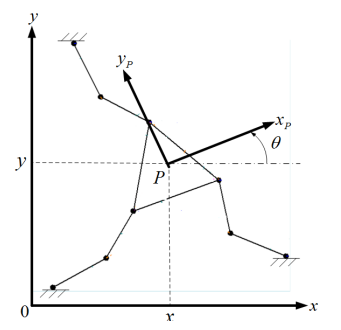
\includegraphics[scale=1]{1.PNG} 
\begin{flushleft}
Para obtener las restricciones cinemáticas del manipulador
se utiliza el método de propagación de velocidades, mostrado en  partiendo del punto P de la plataforma móvil
hasta llegar al inicio de cada cadena (ver Fig. 1). \\
Una vez que se tienen las restricciones cinemáticas de velocidad de cada cadena, la cinemática diferencial del manipulador paralelo puede ser expresada en el sistema inercial por
el sistema de ecuaciones diferenciales de la siguiente forma: At(q)q=0.\begin{flushleft}
Donde, ATp(q)∈R(M.
N)×(3+M.
N)
 es la matriz asociada a la cinemática en el sistema inercial, q∈R3+M.
N es el vector de las
coordenadas de configuración y q∈R3+M.
N es el vector de las
velocidades de configuración, donde M es el número de cadenas y N es el número de actuadores por cadena, siendo:\\
\begin{center}
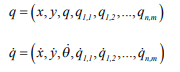
\includegraphics[scale=1]{2.PNG} 
\begin{flushleft}
Para el manipulador 3RRR se tiene que qnm describe la coordenada de configuración de la cadena n de la junta m, donde,
m=1,…, M; n=1,…, N; M=3 y N=3.\\
Por otro lado, si θ=0, es posible encontrar la cinemática
diferencial interna del manipulador, de la siguiente forma:\\
\begin{center}
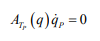
\includegraphics[scale=1]{3.PNG} 
El hecho de que sea interna, se refiere a que está referenciada al sistema local {x P, y P}.\\
Donde ATp(q)∈R(M.
N)×(3+M.
N)
 es la matriz asociada a la cinemática del manipulador expresada en el sistema local {x P, y P}.
El vector qP representa al vector de las velocidades de configuración con respecto al sistema local {x P, y P} siendo:\\
\begin{center}
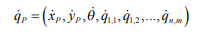
\includegraphics[scale=1]{4.PNG} 
\begin{flushleft}
La Figura 1, muestra la postura del robot paralelo plano
3RRR y se puede describir, como sigue:
\begin{center}
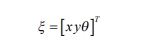
\includegraphics[scale=1]{5.PNG} 
\begin{flushleft}
Donde, la coordenada (x, y) describe la posición del punto
P con respecto al sistema inercial {x, y}y donde θ=θP, es la
orientación del manipulador, medida desde el sistema absoluto al sistema local Además, es el vector postura de velocidades del vector . Sea, el vector postura de velocidades del
vector , expresado en el sistema local , entonces:\\
\begin{flushleft}
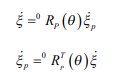
\includegraphics[scale=1]{6.PNG}\\
 Donde: 
 \begin{center}
 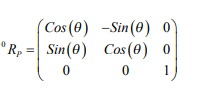
\includegraphics[scale=1]{7.PNG} 
 
 \end{center}
\end{flushleft}
\end{flushleft}
\end{center}
\end{flushleft}
\end{center}
\end{center}
\end{flushleft}
\end{center}
\end{flushleft}
\end{flushleft}
\end{center}
\end{flushleft}
\end{flushleft}
\end{flushleft}
\end{center}
\end{document}